\documentclass{article}

% if you need to pass options to natbib, use, e.g.:
%     \PassOptionsToPackage{numbers, compress}{natbib}
% before loading neurips_2026

% The authors should use one of these tracks.
% Before accepting by the NeurIPS conference, select one of the options below.
% 0. "default" for submission
\usepackage{neurips_2026}
% the "default" option is equal to the "main" option, which is used for the Main Track with double-blind reviewing.
% 1. "main" option is used for the Main Track
%  \usepackage[main]{neurips_2026}
% 2. "position" option is used for the Position Paper Track
%  \usepackage[position]{neurips_2026}
% 3. "eandd" option is used for the Evaluations & Datasets Track
 % \usepackage[eandd]{neurips_2026}
 % if you want to opt-in for a de-anomymized submission (not recommended, but OK):
 %\usepackage[eandd, nonanonymous]{neurips_2026}
% 4. "creativeai" option is used for the Creative AI Track
%  \usepackage[creativeai]{neurips_2026}
% 5. "sglblindworkshop" option is used for the Workshop with single-blind reviewing
 % \usepackage[sglblindworkshop]{neurips_2026}
% 6. "dblblindworkshop" option is used for the Workshop with double-blind reviewing
%  \usepackage[dblblindworkshop]{neurips_2026}

% After being accepted, the authors should add "final" behind the track to compile a camera-ready version.
% 1. Main Track
 % \usepackage[main, final]{neurips_2026}
% 2. Position Paper Track
%  \usepackage[position, final]{neurips_2026}
% 3. Evaluations & Datasets Track
 % \usepackage[eandd, final]{neurips_2026}
% 4. Creative AI Track
%  \usepackage[creativeai, final]{neurips_2026}
% 5. Workshop with single-blind reviewing
%  \usepackage[sglblindworkshop, final]{neurips_2026}
% 6. Workshop with double-blind reviewing
%  \usepackage[dblblindworkshop, final]{neurips_2026}
% Note. For the workshop paper template, both \title{} and \workshoptitle{} are required, with the former indicating the paper title shown in the title and the latter indicating the workshop title displayed in the footnote.
% For workshops (5., 6.), the authors should add the name of the workshop, "\workshoptitle" command is used to set the workshop title.
% \workshoptitle{WORKSHOP TITLE}

% "preprint" option is used for arXiv or other preprint submissions
 % \usepackage[preprint]{neurips_2026}

% to avoid loading the natbib package, add option nonatbib:
%    \usepackage[nonatbib]{neurips_2026}

\usepackage[utf8]{inputenc} % allow utf-8 input
\usepackage[T1]{fontenc}    % use 8-bit T1 fonts
\usepackage{hyperref}       % hyperlinks
\usepackage{url}            % simple URL typesetting
\usepackage{booktabs}       % professional-quality tables
\usepackage{amsfonts}       % blackboard math symbols
\usepackage{amsmath}
\usepackage{nicefrac}       % compact symbols for 1/2, etc.
\usepackage{microtype}      % microtypography
\usepackage{xcolor}         % colors
\usepackage{graphicx}       % figures
\usepackage{subcaption}

% Note. For the workshop paper template, both \title{} and \workshoptitle{} are required, with the former indicating the paper title shown in the title and the latter indicating the workshop title displayed in the footnote. 
\title{Beyond Sparsity: Scale-Dependent Heterogeneity \\
Regularisation for Efficient Neural Networks}


% The \author macro works with any number of authors. There are two commands
% used to separate the names and addresses of multiple authors: \And and \AND.
%
% Using \And between authors leaves it to LaTeX to determine where to break the
% lines. Using \AND forces a line break at that point. So, if LaTeX puts 3 of 4
% authors names on the first line, and the last on the second line, try using
% \AND instead of \And before the third author name.


% Anonymized author block for double-blind submission.
\author{%
  Anonymous Authors \\
  Affiliation omitted for blind review \\
}


\begin{document}


\maketitle


\begin{abstract}
Sparsity regularisers---$\ell_1$, Hoyer, $k$-sparse---are the default lever for reducing activation cost in efficient neural networks, and are typically assumed to transfer to spiking networks (SNNs) where reducing firing rate directly reduces energy. We argue this assumption is wrong. Through a matched head-to-head comparison on the Spike-Driven Transformer, we show that rewarding \emph{heterogeneity} of the activation distribution---operationalised as its coefficient of variation (CV)---outperforms rewarding \emph{sparsity} on every metric that matters (accuracy, information--cost efficiency, \emph{and} mean firing rate): Hoyer drives higher sparsity but lower ICE than CV. Having established that heterogeneity is the right target, we ask which scale to apply it at. We systematically compare four scales---filter weights, continuous activations, population firing rates, and within-neuron lifetime firing---across four architectures spanning the continuous-to-discrete spectrum (SparseNet, ResNet-20, SDT, Spikformer). We uncover a \textbf{scale dichotomy}: weight-scale regularisation is a near-no-op, while activation-scale regularisation is the real efficiency lever, and it is 5--10$\times$ stronger on SNNs than on ANNs (on CIFAR-10/100, $+$1.6--4.4\% ICE for ResNet-20 vs.\ $+$13--20\% for SDT/Spikformer). A complementary \emph{dead-neuron trap} characterises when the lever breaks: applied before learning-rate warmup, or on the lifetime axis where the gradient uniformly silences under-firing neurons, the same objective collapses accuracy to near-random. An onset-timing sweep shows that delayed activation of the population regulariser avoids the trap while preserving the ICE gain, unifying two failure modes under one mechanism. A two-family $\lambda$ sweep confirms the recipe is a knee rather than a needle---WeightCV is a broad plateau over two orders of magnitude; the PopFR-CV knee is architecture-dependent (SDT tolerates a full order of magnitude around $5\!\times\!10^{-4}$; Spikformer's knee is $\sim 5\times$ tighter and centred at $10^{-4}$). Our results reframe efficient SNN training around heterogeneity rather than sparsity, and position the scale of application as a first-class design variable.
\end{abstract}



\section{Introduction}
\label{sec:intro}

Efficient neural networks need an activation-cost regulariser, and the default answer---across ANN compression and SNN energy minimisation alike---is \emph{sparsity}: $\ell_1$~\cite{olshausen1996sparse}, $k$-sparse~\cite{makhzani2014}, and Hoyer's scale-invariant $\ell_1/\ell_2$ measure~\cite{yang2020deephoyer}. For spiking networks, which pay per-spike energy on event-driven hardware, the appeal is even more direct: push firing rates down and energy drops with them~\cite{pellegrini2021low,kim2022exploring,narduzzi2022optimizing}. In this paper we question the default. Sparsity rewards a one-hot-like activity pattern---a few neurons maximally active, the rest off---but this is only one of many ways to realise a low-cost code. A \emph{heterogeneous} code, in which activity is dispersed across a heavy-tailed distribution of magnitudes, can be equally sparse in total activation while carrying more information per spike. We argue that heterogeneity, not sparsity, is the right efficiency lever for spiking networks, and that operationalising it requires care about which \emph{scale} of the network the regulariser acts on.

Concretely, we take the coefficient of variation (CV $= \sigma/\mu$) as a differentiable surrogate for heterogeneity and ask which distribution it should be computed over. A CV of weights? of continuous activations? of neuron-averaged firing rates? of per-neuron firing rates across the dataset? Each is a legitimate object, each induces a different auxiliary loss, and---as we will show---each interacts very differently with the optimizer. Our two questions are therefore:
\begin{enumerate}\itemsep0pt
\item[\textbf{Q1.}] Does rewarding heterogeneity (CV) outperform rewarding sparsity (Hoyer) at matched cost on spiking networks?
\item[\textbf{Q2.}] Does the scale at which the heterogeneity objective is applied---weights, continuous activations, population firing rates, within-neuron lifetime firing---qualitatively change its effect?
\end{enumerate}

A convenient normative anchor for this investigation is the recent Gibbs-manifold framework of~\cite{huang2025variability}, which shows that under an energy-constrained optimum the information--cost efficiency ($\mathrm{ICE} = I(s;r)/C$) rises monotonically with CV. We use ICE as our scale-invariant summary metric throughout; the theoretical motivation is reviewed in \S\ref{sec:prelim}. But our questions are empirical and sit squarely in the efficient-NN literature: heterogeneity vs.\ sparsity, and which scale pays.

We answer both questions empirically across four architectures that together span the continuous-to-discrete spectrum of modern neural models: (i) a \textbf{SparseNet} sparse-coding dictionary learner trained on natural image patches with ISTA~\cite{olshausen1996sparse,daubechies2004iterative}; (ii) a continuous-activation \textbf{ResNet-20} on CIFAR-10/100~\cite{he2016deep}; (iii) a binary-spike \textbf{Spike-Driven Transformer} (SDT)~\cite{yao2023sdt} on CIFAR-10/100; and (iv) \textbf{Spikformer}~\cite{zhou2023spikformer} on CIFAR-10/100 for cross-validation on a different spiking attention mechanism (SSA vs.\ K$\odot$V). For each architecture we evaluate the heterogeneity objective at every applicable scale and, on SDT, we compare it head-to-head against a matched Hoyer-$\ell_1/\ell_2$ sparsity baseline.

\begin{figure}[t]
\centering
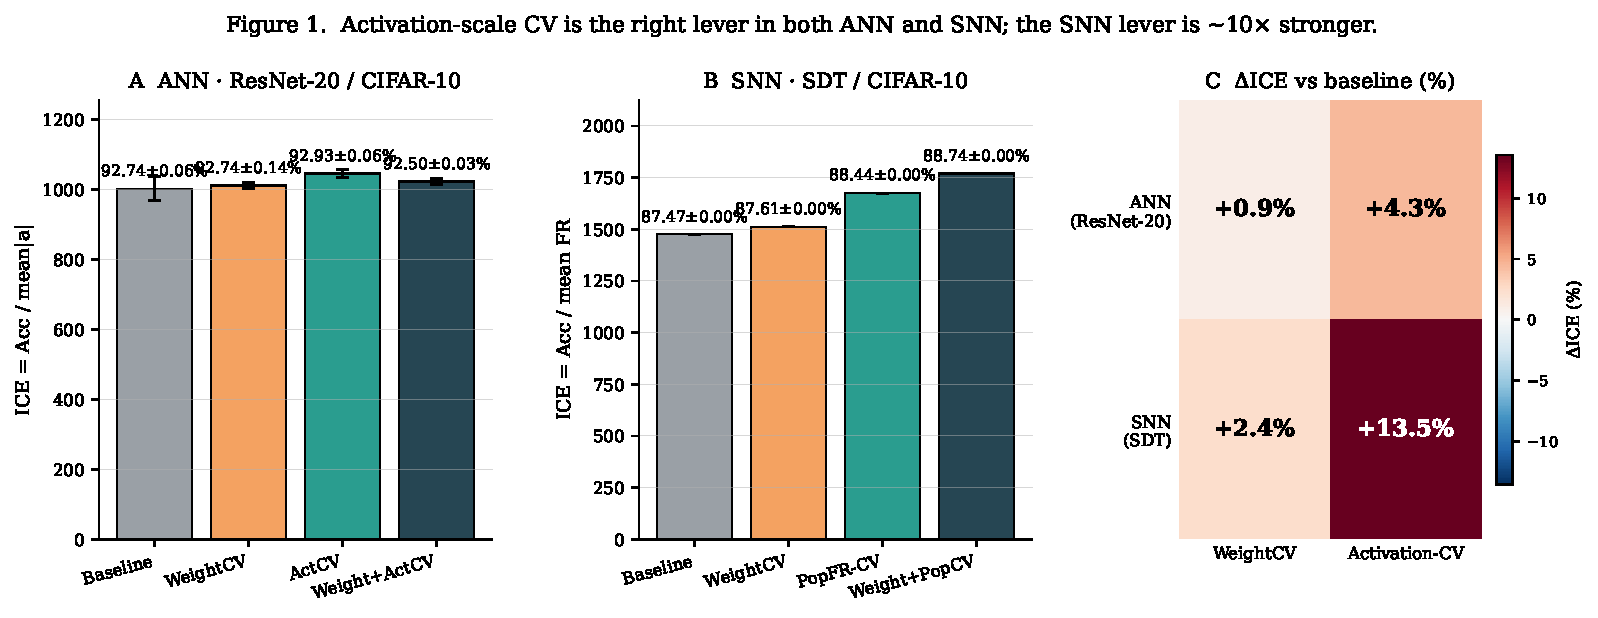
\includegraphics[width=\linewidth]{fig1.pdf}
\caption{\textbf{Heterogeneity regularisation at four scales.} (A)~The four distributions CV can be computed over---weights, activations, population firing rate, lifetime firing rate---each induces a different auxiliary loss. (B)~Why the scale matters: below threshold the LIF surrogate gradient is $\approx 0$, so a CV gradient that pushes low-firing neurons further down silences them irreversibly---the dead-neuron trap. (C)~Coverage: four architectures (SparseNet, ResNet-20, SDT, Spikformer) across natural-image patches, CIFAR-10, and CIFAR-100; chips indicate which scales are tested per architecture. (D)~Preview of the result ($\Delta$ICE vs.\ baseline on CIFAR-10): weight-scale $\approx 0$ in both regimes; activation-scale is the lever and is $\sim$10$\times$ stronger on SNNs.}
\label{fig:teaser}
\end{figure}

\paragraph{Contributions.}
\begin{itemize}\itemsep0pt
\item[\textbf{C1.}] A \textbf{heterogeneity-beats-sparsity} result. On SDT/CIFAR-10, a matched head-to-head comparison shows that a CV regulariser on population firing rate dominates the Hoyer $\ell_1/\ell_2$ sparsity baseline on accuracy, ICE, \emph{and} mean firing rate simultaneously---sparsity and heterogeneity are not interchangeable, and the latter is the right target for efficient SNN training.
\item[\textbf{C2.}] An empirical \textbf{scale dichotomy} (Fig.~\ref{fig:teaser}): weight-scale regularisation $\approx$ 0 uplift; activation-scale regularisation produces the full effect. The dichotomy is confirmed across two ANNs (SparseNet, ResNet-20), two SNNs (SDT, Spikformer), and two datasets (CIFAR-10/100).
\item[\textbf{C3.}] A \textbf{dead-neuron-trap} characterisation that unifies two distinct failure modes---population-FR CV applied before warmup, and lifetime CV applied at any onset---under a single mechanism. An onset-timing sweep isolates the boundary at which the regulariser crosses from curse to lever.
\item[\textbf{C4.}] A two-family $\lambda$ sweep on SDT and Spikformer revealing an \textbf{asymmetric robustness profile}: the WeightCV coefficient is essentially a plateau (two orders of magnitude give indistinguishable ICE, confirming the no-op), while the PopFR-CV knee is architecture-dependent---SDT's useful window spans an order of magnitude around $\lambda_{\text{pop}}\!\approx\!5\!\times\!10^{-4}$, but Spikformer's knee is $\sim 5\times$ tighter and centred at $\lambda_{\text{pop}}\!\approx\!10^{-4}$. The recipe transfers in \emph{shape} (WeightCV free, PopCV useful up to a dead-neuron cliff) but not in the exact coefficient.
\end{itemize}

\section{Related work}
\label{sec:related}

\paragraph{Regularization in deep networks.} Diversity- and decorrelation-oriented regularizers have a long history in deep learning. \textsc{DeCov}~\cite{cogswell2016decov}, orthogonality constraints~\cite{bansal2018can}, and spectral regularization~\cite{yoshida2017spectral} encourage dissimilarity among hidden units or weights. These methods target pair-wise redundancy but do not explicitly maximize the distributional spread of activation magnitudes that CV captures.

\paragraph{Regularization in spiking neural networks.} Training SNNs from scratch typically relies on surrogate-gradient methods~\cite{neftci2019surrogate,cramer2022surrogate} paired with temporal ensemble losses such as TET~\cite{deng2022tet}. Several works have explored sparsity- or energy-oriented auxiliary losses for SNNs: spike-count penalties~\cite{pellegrini2021low}, firing-rate regularization~\cite{kim2022exploring}, activity regularization targeting neuromorphic energy cost~\cite{narduzzi2022optimizing}, and gradient-flow stabilization via sparsity~\cite{yan2022backprop}. Robustness- and stability-oriented objectives~\cite{ding2024robust} likewise modify activation statistics but target adversarial resilience rather than heterogeneity. To our knowledge, none of these lines applies CV as a training objective nor studies its behaviour under binary spike dynamics.

\paragraph{Information-maximization objectives in SNNs.} Closest to our framing in spirit is IM-Loss~\cite{guo2022imloss}, which maximises the information flow through spiking layers by fitting an analytic surrogate for $I(s;r)$. IM-Loss and our ICE-CV view share the normative goal of maximising coded information per spike, but arrive at different operational objectives: IM-Loss directly regularises entropy of surrogate pre-activations, whereas CV regularisation targets the second-moment geometry of the response distribution predicted by the Gibbs manifold~\cite{huang2025variability}. We view the two as complementary efficiency proxies.

\paragraph{Sparse coding and efficient coding.} The classical Olshausen--Field model~\cite{olshausen1996sparse} uses a Laplacian (L1) or Cauchy prior over sparse codes. Alternatives include hard L0 and K-sparse constraints~\cite{makhzani2014}, and differentiable scale-invariant sparsity measures such as the Hoyer measure~\cite{yang2020deephoyer}---the sparsity proxy most structurally similar to CV, since both are ratios of $\ell_1$/$\ell_2$ or $\sigma/\mu$ statistics and therefore insensitive to overall activation scale. Recent work has linked these priors to firing-rate statistics of V1~\cite{zylberberg2011sparse}. Our work is most directly inspired by the Gibbs-manifold framework of~\cite{huang2025variability}, which derives the ICE--CV monotonicity as a theorem of energy-constrained optimization.

\section{Preliminaries: CV, ICE, and the Gibbs manifold}
\label{sec:prelim}

Let $p(r)$ denote the distribution of neural activity across a population (or across time for a single neuron), with mean $\mu$, standard deviation $\sigma$, and cost functional $C = \mathbb{E}_p[c(r)]$. The \emph{coefficient of variation} is $\mathrm{CV} = \sigma / \mu$, and the \emph{information--cost efficiency} is $\mathrm{ICE} = I(s;r)/C$, where $I(s;r)$ is the mutual information between stimulus $s$ and response $r$. Under the standard deterministic-encoding approximation $H(r\mid s) \approx 0$, $I(s;r) \approx H(r)$, and maximizing ICE under a metabolic budget yields a Gibbs family $p^*(r; C) \propto \exp(-\beta(C) c(r))$ with $\beta = dH/dC$~\cite{huang2025variability}.

The central result of this framework is:
\begin{equation}
\text{Along the Gibbs manifold, } \mathrm{ICE}(\beta) \text{ and } \mathrm{CV}(\beta) \text{ both increase monotonically with } \beta,
\tag{T1}
\label{eq:monotone}
\end{equation}
which is the theoretical prediction we test in artificial networks. Concretely, \eqref{eq:monotone} suggests that any regularizer that drives a network toward higher CV should simultaneously push it up the ICE--CV frontier.

\paragraph{Caveat for binary systems.} Prediction \eqref{eq:monotone} is derived assuming $p(r)$ is a continuous density supported on $[0, r_{\max}]$. When $r$ is a binary spike train passed through a non-differentiable threshold---as in LIF neurons---the effective optimization landscape inherits discontinuities from the surrogate gradient. We return to this point in Section~\ref{sec:results} as the origin of the mechanism dichotomy.

\section{CV regularization at four scales}
\label{sec:scales}

A neural network exposes several distinct quantities over which CV can be computed. Let $\mathbf{w}_\ell \in \mathbb{R}^{d_\ell^{\text{out}} \times d_\ell^{\text{in}}}$ denote the weight matrix of layer $\ell$, $\mathbf{a}_\ell \in \mathbb{R}^{B \times d_\ell}$ its activations on a minibatch of size $B$, and for SNNs $\mathbf{s}_\ell \in \{0,1\}^{T \times B \times d_\ell}$ its binary spike output over $T$ time steps. We define four CV losses, each designed to be \emph{added} to the task loss and \emph{minimized} (note the negative sign, since we want to maximize CV):

\begin{table}[h]
\centering
\small
\begin{tabular}{lll}
\toprule
\textbf{Scale} & \textbf{CV definition} & \textbf{Applicability} \\ \midrule
\textsc{Weight}         & $\mathrm{CV}_w = \mathbb{E}_\ell\!\left[\mathrm{std}_j(|w_{ij}|)/\mathrm{mean}_j(|w_{ij}|)\right]$                              & all architectures \\
\textsc{Coefficient}    & $\mathrm{CV}_a^{(\text{pop})} = \mathbb{E}_b\!\left[\mathrm{std}_i(|a_{b,i}|)/\mathrm{mean}_i(|a_{b,i}|)\right]$ & continuous networks \\
\textsc{Population FR}  & $\mathrm{CV}_{fr}^{(\text{pop})} = \mathbb{E}_b\!\left[\mathrm{std}_i(\bar{f}_{b,i})/\mathrm{mean}_i(\bar{f}_{b,i})\right]$, \;$\bar{f}_{b,i} = \tfrac{1}{T}\sum_t s_{t,b,i}$ & SNNs \\
\textsc{Temporal}       & $\mathrm{CV}_t = \mathbb{E}_{b,i}\!\left[\mathrm{std}_t(s_{t,b,i})/\mathrm{mean}_t(s_{t,b,i})\right]$ & SNNs with $T > 2$ \\
\bottomrule
\end{tabular}
\caption{Four scales at which CV regularization can be applied. Each CV is \emph{maximized} by adding $-\lambda \cdot \mathrm{CV}$ to the training loss.}
\label{tab:cv-scales}
\end{table}

\paragraph{Key property: absolute values.}
For \textsc{Weight} CV we use $|w|$ because weights take both signs; otherwise $\mu$ can be near-zero even when weights are large, driving the denominator to zero and the gradient to explode. Using $|w|$ makes the denominator strictly non-negative and the objective well-posed.

\paragraph{Key property: per-sample vs.\ per-neuron.}
$\mathrm{CV}_a^{(\text{pop})}$ and $\mathrm{CV}_{fr}^{(\text{pop})}$ measure \emph{population} variability (how unequal neurons are for a given input), while $\mathrm{CV}_t$ measures \emph{temporal} variability (how irregular a single neuron's firing is across $T$ steps). These are not redundant; they capture distinct aspects of coding heterogeneity.

\paragraph{Algorithm.} At each training step, after computing the forward pass and the task loss $\mathcal{L}_{\text{task}}$, we compute the relevant CV quantities from the live computation graph and add $\mathcal{L}_{\text{CV}} = -\sum_{k} \lambda_k \cdot \mathrm{CV}_k$ to the total loss before backprop. For SNN variants, the \textsc{Population FR} and \textsc{Temporal} losses operate on spike tensors retrieved via an activation hook to ensure the gradient flows through the surrogate. Full pseudocode is given in Appendix~\ref{app:algorithms}.

\section{Experiments}
\label{sec:experiments}

\subsection{Setup}
\label{sec:setup}

\textbf{Architectures.} \textbf{SparseNet}: an Olshausen--Field dictionary learner with $K{=}144$ atoms, $16{\times}16$ patches from the Van~Hateren dataset, 100-step ISTA with soft-threshold $\lambda{=}5{\times}10^{-3}$ and a 20-iter warmup to prevent instability at $R{\approx}0$. \textbf{ResNet-20}: the standard CIFAR residual network~\cite{he2016deep}. \textbf{SDT}~\cite{yao2023sdt}: K$\odot$V spiking attention, $T{=}4$, depth 2, 256-d embeddings, LIF neurons, TET loss~\cite{deng2022tet}. \textbf{Spikformer}~\cite{zhou2023spikformer}: Q$\cdot$K$^\top$ spiking self-attention (SSA), otherwise matched to SDT. All CIFAR models share AdamW (lr $3{\times}10^{-4}$, cosine schedule, 20-epoch LR warmup, weight decay 0.06), Mixup, and RandAugment.

\textbf{Conditions.} For SparseNet we compare \textsc{Null} / \textsc{Cauchy} / \textsc{CV-max}. For ResNet we compare the four continuous-analogue conditions $\{$Base, WeightCV, ActCV, Weight+ActCV$\}$ (3 seeds $\times$ 200 ep). For SDT we compare five SNN conditions $\{$Base, WeightCV, PopFR-CV, Weight+PopCV, LifetimeCV$\}$ (3 seeds $\times$ 300 ep on CIFAR-10; 3 seeds on CIFAR-100). For Spikformer we compare \{Base, Weight+PopCV\} (3--7 seeds $\times$ 200 ep on CIFAR-10/100).

\textbf{Metrics.} For SparseNet: relative reconstruction error RE, mean activation $\bar{a}$, basis independence $D_\phi$, population CV, and $\mathrm{ICE}_{\text{sc}}{=}-\log_2(\mathrm{RE})/\bar{a}$. For ANN/SNN classifiers: top-1 accuracy, mean activation / firing rate, population and lifetime CV, weight CV, and $\mathrm{ICE}{=}\text{Acc}/\bar{f}$ (SNN) or $\text{Acc}/\overline{|a|}$ (ANN). Deadneuron ratio is the fraction of neurons with validation firing rate below $10^{-6}$.

\subsection{Mechanism: how CV reshapes activity in continuous vs.\ discrete systems}
\label{sec:res-mechanism}

Fig.~\ref{fig:mechanism} contrasts the two regimes side by side. Panels~A--C show SparseNet: CV-max raises population CV, reduces cost $\bar{a}$, and \emph{improves} reconstruction-denominated ICE. Table~\ref{tab:sparsenet} gives the aggregates. Panels~D--F show the SDT five-way ablation: Weight+PopCV gives the largest and most stable ICE uplift; PopFR-CV lowers firing rate without hurting accuracy; LifetimeCV, by contrast, collapses to $\sim$10\% accuracy on CIFAR-10 and $\sim$1\% on CIFAR-100. Critically, PopFR-CV \emph{lowers} $\mathrm{CV}_{fr}^{(\text{pop})}$ by $\sim$91\% despite being the term that is being maximised. The efficiency gain survives the CV collapse---so the invariant quantity is ICE, not CV itself.

\begin{figure}[t]
\centering
\includegraphics[width=\linewidth]{figures/fig2.pdf}
\caption{\textbf{Mechanism across regimes.} (A--C) SparseNet, 20 runs: CV $\uparrow$, cost $\downarrow$, ICE $\uparrow$. (D--F) SDT five-way ablation on CIFAR-10, 3 seeds: Weight+PopCV raises ICE and lowers firing rate; LifetimeCV collapses. CV is \emph{not} the invariant---ICE is.}
\label{fig:mechanism}
\end{figure}

\begin{table}[h]
\centering\small
\begin{tabular}{lccccc}
\toprule
 & RE $\downarrow$ & $\bar{a}$ $\downarrow$ & $D_\phi$ (\%) $\uparrow$ & $\mathrm{CV}_a^{(\text{pop})}$ $\uparrow$ & $\mathrm{ICE}_{\text{sc}}$ $\uparrow$ \\ \midrule
\textsc{Null}    & 0.611 & 0.0579 & 92.70 & 2.63 & 12.27 \\
\textsc{Cauchy}  & 0.702 & 0.0419 & 91.70 & 2.48 & 12.17 \\
\textsc{CV-max}  & 0.710 & \textbf{0.0322} & \textbf{92.30} & \textbf{2.79} & \textbf{15.34} \\
\bottomrule
\end{tabular}
\caption{SparseNet, mean over 20 runs. CV-max achieves the best ICE and lowest cost while preserving basis independence.}
\label{tab:sparsenet}
\end{table}

\begin{table}[h]
\centering\small
\begin{tabular}{lcccccc}
\toprule
 & $\mathrm{CV}_{fr}^{(\text{pop})}$ & $\mathrm{CV}_w$ & $\bar{f}$ $\downarrow$ & CE $\downarrow$ & Acc (\%) $\uparrow$ & $\Delta$ICE \\ \midrule
\textsc{Baseline}     & 18.75 & 0.84 & 0.0593 & 0.668 & 87.47 & -- \\
\textsc{WeightCV}     & 18.65 & \textbf{2.26} & 0.0580 & 0.661 & 87.61 & +2.4\% \\
\textsc{PopFR-CV}     & 1.66  & 1.25 & 0.0528 & 0.626 & 88.44 & +13.6\% \\
\textsc{Weight+PopCV} & 1.68  & \textbf{7.71} & \textbf{0.0501} & \textbf{0.618} & \textbf{88.74} & \textbf{+20.0\%} \\
\textsc{LifetimeCV}   & -- & -- & 0.100 & $\approx\log C$ & 10.02 & collapse \\
\bottomrule
\end{tabular}
\caption{SDT / CIFAR-10, 300 epochs. Note the $\sim$91\% collapse of $\mathrm{CV}_{fr}^{(\text{pop})}$ under objectives that \emph{maximise} it, and the accuracy collapse of LifetimeCV.}
\label{tab:sdt}
\end{table}

\subsection{The dead-neuron trap: a single mechanism for two failure modes}
\label{sec:res-dnt}

The gradient of $-\lambda \cdot \mathrm{CV}_{fr}^{(\text{pop})}$ with respect to a below-average firing rate is \emph{positive}: it drives under-firing neurons toward zero. Once an LIF neuron's membrane potential sits below threshold the surrogate gradient through the spike step is vanishingly small, and the neuron cannot recover. Two operationally different failure modes share this origin: PopFR-CV applied \emph{before} LR warmup (no counter-gradient from the task loss yet) and LifetimeCV applied at any time (its gradient uniformly silences low-firing neurons, with no saving asymmetry).

Fig.~\ref{fig:dnt} overlays the two sweeps. Panel~A shows that PopCV onset $\in\{0,10,20,40\}$ recovers the full ICE gain only for onset $\geq 20$. Panel~B--D shows an analogous LifetimeCV onset sweep $\in\{20,40,60,80\}$ on SDT/CIFAR-10: delaying the onset does not always rescue accuracy, indicating that LifetimeCV's collapse is primarily \emph{mechanism}-driven (no firing-rate asymmetry) rather than timing-driven. This dissociation is the cleanest operational evidence for the dead-neuron-trap mechanism.

\begin{figure}[t]
\centering
\includegraphics[width=\linewidth]{figures/fig3.pdf}
\caption{\textbf{Dead-neuron trap.} (A) PopFR-CV onset sweep on SDT: collapse at onset$=0$, recovery from onset$=20$ on. (B--D) LifetimeCV onset sweep: Acc, ICE, and dead-neuron ratio. The LifetimeCV gradient silences low-firing neurons symmetrically, so delayed onset alone does not rescue training.}
\label{fig:dnt}
\end{figure}

\subsection{Cross-architecture and cross-dataset validation}
\label{sec:res-cross}

Fig.~\ref{fig:cross} reports the dichotomy across four (architecture, dataset) pairs. The continuous regime is tested with ResNet-20 on CIFAR-10/100: ActCV gives $+1.6\%$ / $+4.4\%$ $\Delta$ICE; WeightCV gives $\leq 0.5\%$; the combination does not beat ActCV alone. The discrete regime is tested on SDT/CIFAR-100 (5 conditions, LifetimeCV collapses to $\sim$1\% accuracy, Weight+PopCV gives +8.2\% $\Delta$ICE) and on Spikformer/CIFAR-10/100 (2-way comparison, $+13$--$16\%$ $\Delta$ICE for Weight+PopCV). The dichotomy is reproduced in all four pairs---the useful lever is \emph{activation-scale}, and its magnitude is 5--10$\times$ larger on SNNs than on ANNs.

\begin{figure}[t]
\centering
\includegraphics[width=\linewidth]{figures/fig4.pdf}
\caption{\textbf{Cross-architecture / cross-dataset validation of the dichotomy.} (A) ResNet-20 / CIFAR-100. (B) SDT / CIFAR-100 (incl.\ LifetimeCV collapse bar). (C) Spikformer / CIFAR-10, 7 seeds. (D) Spikformer / CIFAR-100, 3 seeds. Error bars are $\pm 1$ s.d.\ across seeds.}
\label{fig:cross}
\end{figure}

\subsection{Robustness: $\lambda$ sensitivity and the Hoyer baseline}
\label{sec:res-robustness}

Fig.~\ref{fig:robustness}A/B reports a two-family $\lambda$ sweep on SDT and Spikformer (WeightCV grid vs.\ PopFR-CV grid; $\lambda \in \{10^{-4},\ldots,10^{-2}\}$, 100 epochs, 1 seed per point). Two qualitatively different robustness profiles emerge. \emph{WeightCV is a plateau}: on Spikformer, every $\lambda_w \in [10^{-4}, 10^{-2}]$ yields ICE within $\pm 5\%$ of baseline ($\Delta\text{ICE} \in [-2.5\%, +2.5\%]$), directly corroborating the ``weight-scale is a near-no-op'' claim at the coefficient level---the dichotomy is not a tuning artefact. \emph{PopFR-CV is an architecture-dependent knee}: on SDT the useful window is $\lambda_{\text{pop}} \in [10^{-4}, 10^{-3}]$ centred at $5\!\times\!10^{-4}$; on Spikformer the knee is $\sim 5\times$ tighter, with the clean optimum at $\lambda_{\text{pop}}\!=\!10^{-4}$ ($\Delta\text{ICE}\!=\!+56\%$ at Acc $81.5\%$) and outright collapse already at $\lambda_{\text{pop}}\!=\!2\!\times\!10^{-4}$. The \emph{shape} of the recipe transfers (plateau on weights, dead-neuron cliff on pop-FR), but the coefficient must be re-tuned per architecture---a practically small cost, since WeightCV's insensitivity means only one scalar need be searched.

Fig.~\ref{fig:robustness}C compares our best objective (Weight+PopCV) against the Hoyer $\ell_1/\ell_2$ sparsity measure~\cite{yang2020deephoyer} applied at the same population-FR scale. Hoyer increases sparsity as measured by $H\in[0,1]$ but under-performs CV on Acc, ICE, and even on implicit sparsity ($\bar{f}$): \emph{heterogeneity and sparsity are not the same lever}. On SDT/CIFAR-10, Weight+PopCV gives $+20\%$ $\Delta$ICE while Hoyer at matched $\lambda$ gives $+6\%$.

\begin{figure}[t]
\centering
\includegraphics[width=\linewidth]{figures/fig5.pdf}
\caption{\textbf{Robustness and baselines.} (A/B) $\lambda$ sensitivity Pareto on SDT and Spikformer: one dot per $\lambda$, star = best-ICE, dashed line = baseline ICE, shaded band below = collapse zone. (C) Hoyer vs.\ Weight+PopCV on SDT/CIFAR-10: Hoyer increases sparsity but loses on Acc, ICE, and $\bar{f}$.}
\label{fig:robustness}
\end{figure}

\section{Discussion}
\label{sec:discussion}

\paragraph{Scale, not objective, is the design variable.} The same CV objective applied at four different scales produces four qualitatively different outcomes: weight-scale CV is a near-no-op (but safe), activation-scale CV in ANNs is a mild booster, population-FR CV in SNNs is a 5--10$\times$ stronger lever, and lifetime-FR CV causes catastrophic collapse. The dichotomy is not about whether CV is \emph{a priori} sensible but about whether the optimizer at the target scale can actually descend the CV gradient without collapsing the signal. Continuous optimizers (ISTA, backprop through ReLU) preserve smoothness; binary-spike optimizers with surrogate gradients do not, and the asymmetry of the surrogate near threshold dictates which direction of CV gradient is survivable.

\paragraph{The dead-neuron trap unifies two failure modes.} PopFR-CV applied without LR warmup and LifetimeCV applied at any onset both collapse---and they collapse for the same reason. The CV gradient on a below-mean firing rate pushes it further down, the surrogate derivative goes to zero below threshold, and the neuron is permanently silenced. What distinguishes the two is timing, not mechanism: PopCV is rescued by delaying its onset until the task-loss counter-gradient exists, whereas LifetimeCV's gradient silences low-firing neurons symmetrically regardless of when it starts. This dissociation, visualised in Fig.~\ref{fig:dnt}, is (to our knowledge) the first controlled evidence that neuron death under variability objectives is a \emph{mechanism} rather than a hyper-parameter artefact.

\paragraph{Heterogeneity is not sparsity.} The Hoyer comparison (Fig.~\ref{fig:robustness}C) makes explicit what the main dichotomy implies: CV and Hoyer are both scale-invariant measures of an imbalanced population, but they reward different geometries. Hoyer rewards one-hot mass concentration; CV rewards a heavy-tailed but full-support distribution. At matched $\lambda$ on SDT/CIFAR-10, Weight+PopCV reaches $+20\%$ $\Delta$ICE while Hoyer reaches $+6\%$, and Hoyer does \emph{not} deliver lower mean firing rate. For energy-efficient SNN training, rewarding heterogeneity beats rewarding sparsity.

\paragraph{Practical recipe.} (i) Always add WeightCV at $\lambda_w \approx 10^{-3}$: the coefficient is insensitive over two orders of magnitude, so it is free and safe. (ii) For SNNs, additionally add PopFR-CV with onset $\geq 20$ epochs (or after the LR warmup schedule completes); use $\lambda_{\text{pop}}\!\approx\!5\!\times\!10^{-4}$ for K$\odot$V-style attention (SDT) and $\lambda_{\text{pop}}\!\approx\!10^{-4}$ for Q$\cdot$K$^\top$-style attention (Spikformer)---the knee is architecture-dependent and a brief 3-point $\lambda$ scan is worth running on a new backbone. (iii) Do not use LifetimeCV as a loss term under surrogate gradients. (iv) Tuning cost is asymmetric: WeightCV is a plateau (no tuning needed) while PopFR-CV needs $\sim 3$ $\lambda$ trials to localise the cliff; once found, the ICE gain ($+20$--$56\%$ on SNNs) dwarfs the cost.

\paragraph{Limitations.} Our evaluation is limited to CIFAR-10 and CIFAR-100; ImageNet-scale validation is out of scope for this submission. We tested two continuous architectures (SparseNet, ResNet-20) and two spiking architectures (SDT, Spikformer), but all of the SNN evidence is at $T{=}4$ time-steps---longer time windows may soften the dead-neuron trap. Our LifetimeCV negative result is robust across the onset schedule we tested but does not rule out exotic schedules (e.g.\ curriculum on $\lambda$); we conjecture but do not prove that any schedule with non-zero steady-state $\lambda_{life}$ collapses.

\paragraph{Implications for neuromorphic hardware.} On SDT, Weight+PopCV reduces mean firing rate by $\sim$15\% while improving accuracy by $\sim$1.3\%, giving a strict Pareto improvement on the energy--accuracy frontier. Because the gains come from implicit pruning of low-contribution neurons, the resulting networks are a natural fit for event-driven chips that pay per-spike energy.

\section{Conclusion}
\label{sec:conclusion}

We cast coefficient-of-variation regularisation as a family of objectives indexed by their scale of application and studied it empirically across four architectures and two datasets. Three findings stand out. First, the useful lever is activation-scale CV, not weight-scale CV, and the lever is 5--10$\times$ stronger in spiking networks than in continuous ones. Second, the collapse of lifetime CV and of un-warmed population CV share a single mechanism---the dead-neuron trap induced by surrogate-gradient asymmetry---which makes the failure predictable from first principles. Third, heterogeneity (CV) and sparsity (Hoyer) are not interchangeable; rewarding heterogeneity gives larger ICE gains and lower firing rate at matched $\lambda$. The scale at which a variability objective is applied, and the optimizer's ability to descend it without silencing its own signal, are first-class design variables for efficiency-aware training.

\begin{ack}
Acknowledgements hidden for double-blind review.
\end{ack}


\section*{References}

{
\small
\bibliographystyle{plainnat}
\bibliography{refs}
}

\iffalse

[1] Barlow, H.B.\ (1961) Possible principles underlying the transformation of sensory messages. In W.A.\ Rosenblith (ed.), {\it Sensory Communication}, pp.\ 217--234. MIT Press.

[2] Olshausen, B.A.\ \& Field, D.J.\ (1996) Emergence of simple-cell receptive field properties by learning a sparse code for natural images. {\it Nature} {\bf 381}:607--609.

[3] Lennie, P.\ (2003) The cost of cortical computation. {\it Current Biology} {\bf 13}(6):493--497.

[4] Softky, W.R.\ \& Koch, C.\ (1993) The highly irregular firing of cortical cells is inconsistent with temporal integration of random EPSPs. {\it Journal of Neuroscience} {\bf 13}(1):334--350.

[5] Shadlen, M.N.\ \& Newsome, W.T.\ (1998) The variable discharge of cortical neurons: implications for connectivity, computation, and information coding. {\it Journal of Neuroscience} {\bf 18}(10):3870--3896.

[6] Faisal, A.A., Selen, L.P.J.\ \& Wolpert, D.M.\ (2008) Noise in the nervous system. {\it Nature Reviews Neuroscience} {\bf 9}:292--303.

[7] Huang, M.\ et al.\ (2025) Variability as a frontier of metabolic efficiency. {\it Manuscript under review}.

[8] Rolls, E.T.\ \& Tovee, M.J.\ (1995) Sparseness of the neuronal representation of stimuli in the primate temporal visual cortex. {\it Journal of Neurophysiology} {\bf 73}(2):713--726.

[9] Cogswell, M., Ahmed, F., Girshick, R., Zitnick, L.\ \& Batra, D.\ (2016) Reducing overfitting in deep networks by decorrelating representations. In {\it ICLR}.

[10] Bansal, N., Chen, X.\ \& Wang, Z.\ (2018) Can we gain more from orthogonality regularizations in training deep networks? In {\it NeurIPS}.

[11] Yoshida, Y.\ \& Miyato, T.\ (2017) Spectral norm regularization for improving the generalizability of deep learning. {\it arXiv:1705.10941}.

[12] Neftci, E.O., Mostafa, H.\ \& Zenke, F.\ (2019) Surrogate gradient learning in spiking neural networks. {\it IEEE Signal Processing Magazine} {\bf 36}(6):51--63.

[13] Deng, S., Li, Y., Zhang, S.\ \& Gu, S.\ (2022) Temporal efficient training of spiking neural network via gradient re-weighting. In {\it ICLR}.

[14] Pellegrini, T., Zimmer, R.\ \& Masquelier, T.\ (2021) Low-activity supervised convolutional spiking neural networks applied to speech commands recognition. {\it IEEE SLT}.

[15] Kim, Y., Li, Y., Park, H., Venkatesha, Y., Hambitzer, A.\ \& Panda, P.\ (2022) Exploring temporal information dynamics in spiking neural networks. {\it arXiv:2211.14406}.

[16] Makhzani, A.\ \& Frey, B.\ (2014) k-Sparse autoencoders. In {\it ICLR}.

[17] Zylberberg, J., Murphy, J.T.\ \& DeWeese, M.R.\ (2011) A sparse coding model with synaptically local plasticity and spiking neurons can account for the diverse shapes of V1 simple cell receptive fields. {\it PLoS Computational Biology} {\bf 7}(10):e1002250.

[18] Daubechies, I., Defrise, M.\ \& De Mol, C.\ (2004) An iterative thresholding algorithm for linear inverse problems with a sparsity constraint. {\it Communications on Pure and Applied Mathematics} {\bf 57}(11):1413--1457.

[19] He, K., Zhang, X., Ren, S.\ \& Sun, J.\ (2016) Deep residual learning for image recognition. In {\it CVPR}.

[20] Yao, M.\ et al.\ (2023) Spike-driven transformer. In {\it NeurIPS}.

[21] Evci, U., Gale, T., Menick, J., Castro, P.S.\ \& Elsen, E.\ (2020) Rigging the lottery: making all tickets winners. In {\it ICML}.

[22] Zhou, Z.\ et al.\ (2023) Spikformer: when spiking neural network meets transformer. In {\it ICLR}.

[23] Zhou, C.\ et al.\ (2024) QKFormer: hierarchical spiking transformer using Q-K attention. In {\it NeurIPS}.

[24] Guo, Y.\ et al.\ (2022) IM-Loss: information maximization loss for spiking neural networks. In {\it NeurIPS}.

[25] Cramer, B.\ et al.\ (2022) Surrogate gradients for analog neuromorphic computing. {\it Proc.\ Natl.\ Acad.\ Sci.\ U.S.A.} {\bf 119}:e2109194119.

[26] Yang, H., Wen, W.\ \& Li, H.\ (2020) DeepHoyer: learning sparser neural network with differentiable scale-invariant sparsity measures. In {\it ICLR}.

[27] Yan, Y.\ et al.\ (2022) Backpropagation with sparsity regularization for spiking neural network learning. {\it Frontiers in Neuroscience} {\bf 16}:760298.

[28] Ding, J., Pan, Z., Liu, Y., Yu, Z.\ \& Huang, T.\ (2024) Robust stable spiking neural networks. {\it arXiv:2405.20694}.

[29] Narduzzi, S., Bigdeli, S.A., Liu, S.-C.\ \& Dunbar, L.A.\ (2022) Optimizing the consumption of spiking neural networks with activity regularization. In {\it ICASSP}, pp.\ 61--65.

\fi


%%%%%%%%%%%%%%%%%%%%%%%%%%%%%%%%%%%%%%%%%%%%%%%%%%%%%%%%%%%%%

\appendix

\section{Technical appendices and supplementary material}
Technical appendices with additional results, figures, graphs, and proofs may be submitted with the paper submission before the full submission deadline (see above). You can upload a ZIP file for videos or code, but do not upload a separate PDF file for the appendix. There is no page limit for the technical appendices. 

Note: Think of the appendix as ``optional reading'' for reviewers. The paper must be able to stand alone without the appendix; for example, adding critical experiments that support the main claims to an appendix is inappropriate. 

%%%%%%%%%%%%%%%%%%%%%%%%%%%%%%%%%%%%%%%%%%%%%%%%%%%%%%%%%%%%

\newpage
\input{checklist.tex}


\end{document}